\documentclass[a4paper,12pt]{article}
\usepackage[utf8]{inputenc}
%\usepackage{authblk}
\usepackage{mathtools}
\usepackage{graphicx}
\usepackage{subcaption}

\begin{document}

% Keywords command
\providecommand{\keywords}[1]
{
  \small	
  \textbf{\textit{Keywords---}} #1
}

\title{GPU virtualization in Kernel Based VM}
\author{Liang Yan \textless lyan@suse.com\textgreater}
\date{}
\maketitle
\keywords{GPU Virtualization, KVM, Mdev, SRIOV, VFIO}

\section{Introduction}
Graphics Processing Unit (GPU) has become a powerful platform today, not only providing hardware acceleration for 3D graphic and video encode/decode, but also providing significant performance benefits to big data and machine learning applications due to the development of GPGPU (General-Purpose Computation on GPU). 

On the other hand, system virtualization, as the engine of Cloud, becomes a standard norm for data center today. It can improve resource utilization by running multiple guest machines in one node, it also improves the security and ease of management better than a bare metal machine\cite{kvm}.

With the recent advances in both virtualization and GPU technology, there is a huge demand to support GPU virtualization, make full use of all the advantage of virtualization on GPU. And indeed, GPU virutalization has been implemented in all vendors with most of the  hypervisor already, such as vSpehere and Xenserver, even open source platform KVM.

In this paper, we present an extensive analysis of GPU virtualization techniques based on KVM. We first review  techniques related to GPU virtualization. We then classify GPU virtualization according to the different implementation, from emulated device, API forwarding, device passthrough to full virtualization. Then, we will focus on the full virtualization, and give a full explanation of the key techniques about it. At Last we will checkout the future challenge. 

\section{Background}

\subsection{Modern GPU resource management model\cite{184002}}

\begin{figure}
\centering
  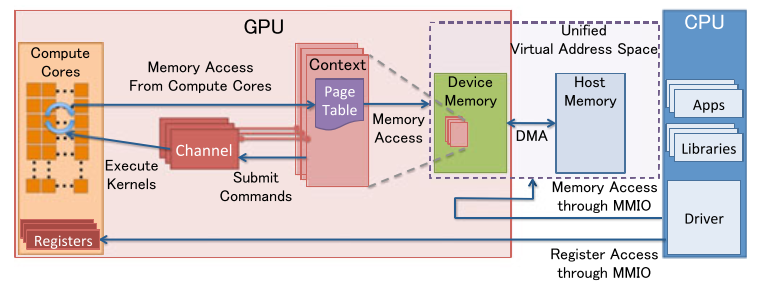
\includegraphics[width=\linewidth]{gpu_management_model.png}
  \caption{GPU resource management model}
  \label{fig:gpuarch}
\end{figure}

From Figure \ref{fig:gpuarch}, Modern GPU resource is consisted of GPU memory, GPU channels, all kinds of Registers and its compute cores.

A GPU has its discrete on-board memory, called GPU RAM. GPU RAM is usually mapped to system memory so that applications can use it as a normal system memory. There is also a DMA connecting system RAM and GPU RAM for large data transfer. For the unified memory architecture (UMA), GPU shares the virtual address space with the CPU process. A page table maintains a mapping between the GPU virtual address to GPU physical address or system physical address, and it uses a tag bit in a page table entry indicating to determine the type.

As a PCI devices, GPU also has a set of registers for configuration space. The operating system recognizes GPU through this configuration space, such as vendor ID, device ID, class etc. Its Base address register (BAR) is used to inform the base address of the mapped memory, which is called BAR memory. The BAR is configured by system firmware at the boot time. The communication between operating system or device driver with I/O devices is usually through Memory-Mapped I/O (MMIO), which is also located on BAR memory. 

The GPU commands are submitted by a special engine called PFIFO, which maintains multiple independent command queues, known as channels. A command queue is a ring buffer with the put and get pointers.A user program can submit commands to the assigned channel. All accesses to channel control area are intercepted by PFIFO engine for execution. GPU driver uses a channel descriptor to store the settings for associated channel, such as
pointers to command buffer, etc.

GPU Context is a logic concept for resource switching, it represents the state of the GPU computing, it also owns a virtual address space in the GPU. Multiple active contexts can coexist on the GPU.

The GPU context is assigned by the GPU page table, which isolates the virtual address space from the others. The GPU page table is separated from the CPU page table. Resides in the GPU memory and its physical address is in a GPU channel descriptor. All the commands and programs submitted through the channel are executed in the corresponding GPU virtual address space.

\subsection{GPU APIs}
Modern GPU uses programmable unified shader architecture today, and it is programmed by below libraries\cite{Dowty:2009:GVV:1618525.1618534}:

Direct3D is a API that provides functions to render two-dimensional (2D) and three-dimensional (3D) graphics, and uses hardware acceleration if available on the graphics card. It is used on the Windows platform only.

OpenGL is an open standard API that provides similiar functions to render 2D and 3D graphics, and is available on most modern operating systems including Windows, macOS, and Linux.

OpenCL is an open standard for cross-platform, parallel programming on heterogeneous system consisting of CPUs, GPUs, digital signal processors (DSPs) and other types of processors or hardware accelerators. 

CUDA is a parallel computing platform introduced by Nvidia. It offers a rich API and set of language extensions that can be used to perform computations on CUDA-enabled GPUs. CUDA could only be used on Nvidia Cards.

\subsection{Kernel-based Virtual Machine}

Kernel-based Virtual Machine is a full virtualization framework for Linux combined with hardware-assisted virtualization. Different with other hypervisor, the main idea of KVM is turning Linux into a hypervisor by adding the KVM kernel module. The other functionality in a system VM can be adapted from the Linux kernel, such as the scheduler, memory management, and I/O subsystems\cite{kvm}.

KVM leverages hardware-assisted virtualization to aginst a pure trap-and-emulation scheme of system virtualization on the x86 architecture, not only allowing the execution of unmodified OSs but also improving the performance in virtualizing CPUs and the memory management unit. The KVM kernel component has been included in the mainline Linux kernel since version 2.6.20 and has become the main virtualization solution in Linux today. 

\subsection{ Direct I/O virtualization technology}

Direct I/O virtualization provides a hardware mechanisms for building a virtualized environment with complete device data transfer isolation, different implementations have been provided, such as  Intel VT-d \cite{vtd}, AMD IOMMU \cite{iommu}, and PCI-SIG IOV\cite{iov}. VT-d and IOMMU are similar. They ensure the isolation I/O address space between different VMs. An I/O MMU similar to MMU installed on PCI bridge to map DMA address to machine memory address. And an IOTLB accelerate this translation. PCI-SIG IOV includes ATS (Address Translation Services), SR-IOV (Single Root IOV), MR-IOV (Multi-Root IOV)\cite{sriov}. 

\subsection{VFIO Platform}

The VFIO driver framework provides unified APIs for direct device access in user-space level. It makes full usage of DMA remapping and Interrupt remapping, exposes direct device access to user space in a secure, IOMMU-protected environment. It provides a low latency and high bandwidth access for guest drivers.\cite{vfio} 

\subsection{MDEV Platform\cite{mdev}}
\begin{figure}
\centering
  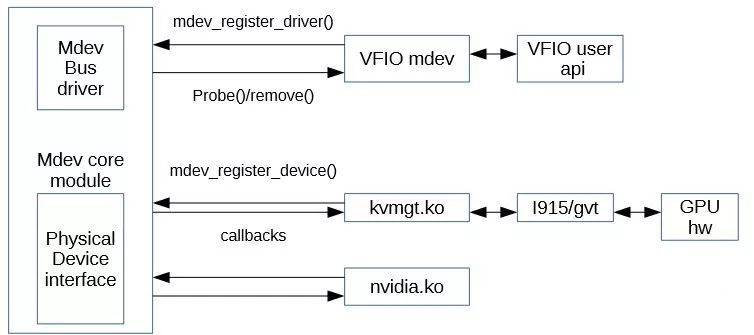
\includegraphics[width=\linewidth]{mdev.png}
  \caption{Mdev Platform Overview}
  \label{fig:mdev}
\end{figure}

MDEV platform is a platform device for the devices that do not have built-in SR-IOV capability.
It provides a unified management interface for such devices by identifying common requirements. 

This framework reuses vfio access mechanism, and it could be used for multiple devices, such as GPUs, network adapters, and compute accelerators. 

The mediated core driver provides a common interface for mediated device management that can be used by drivers of different devices(Figure \ref{fig:mdev}). This module provides a generic interface to perform these operations:

Create and destroy a mediated device

Add a mediated device to and remove it from a mediated bus driver

Add a mediated device to and remove it from an IOMMU group

\section{Classification}
According to different implementation, GPU virtualization usually classify into Software Emulation, API Remoting, Devices Passthrough and Full Virtualization.  

\subsection{Software Emulation}
Emulating a full functional GPU, purely through software, is impractical due to complexity and extremely low performance. Qemu emulates only the legacy VGA cards, with a para-virtualized frame bufferto accelerate 2D specific frame buffer accesses.

Currently, QEMU has emulated five VGA cards, which are VGA, Cirrus, QXL, VMVGA and XEN.

\subsection{API Remoting}
\begin{figure}
  \centering
  \begin{subfigure}[b]{0.4\linewidth}
    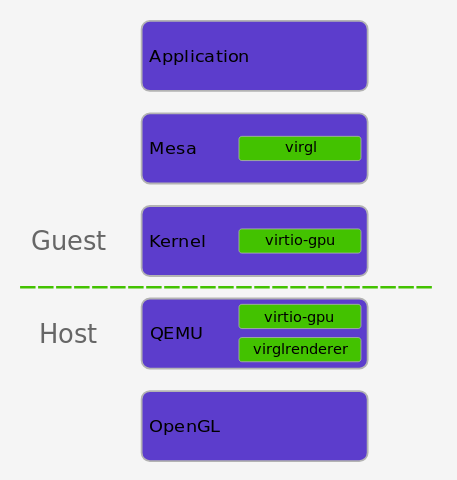
\includegraphics[width=\linewidth]{virtio-gpu.png}
     \caption{virtio-gpu}
  \end{subfigure}
  \begin{subfigure}[b]{0.4\linewidth}
    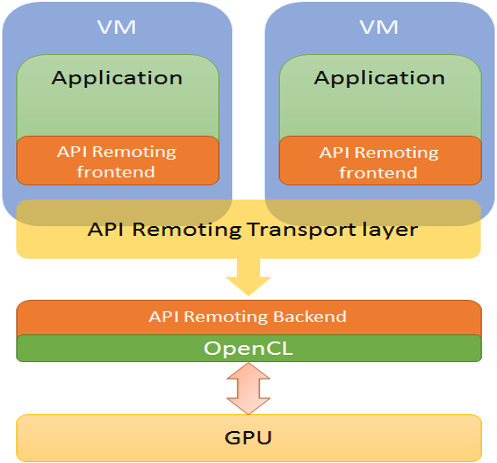
\includegraphics[width=\linewidth]{api_remoting.png}
    \caption{API remoting}
  \end{subfigure}
  \caption{API remoting}
  \label{fig:apiforwarding}
\end{figure}

API Remoting is a high level application implementation, it could intercept API calls from Guest VM directly, and then forward them to host for acceleration. However cost will be huge if APIs are updated in the future. 

Virtio-GPU is an improved API remoting developed by QEMU, it takes the advantage of para virtualization virtio device, forwarding openGL commands from guet to host, which is much faster than those RPC or network protocol implementation.    

\subsection{Device Passthrough}

Based on the VT-d and VFIO techniques above, KVM could passthrough the GPU to exactly one VM, it will translate io address of VM  and re-map its DMA to host address directly, comes along with user-space interface VFIO, it could provide native-close performance.   

\subsection{Full virtualization of GPU}

Full virtualization of GPU means GPU could have full features for each VM, and VMs do not need to change driver for library compatible, and most importantly it could still have high performance. 

Three major vendors all have implemented Full virtualization today.

AMD provides Multiuser GPU with SRIOV (Single Root I/O virtualization) based GPU virtualization.

Nvidia GRID technology uses a vGPU manager to share GPU based on time slices. The graphics commands of each VM are passed directly to the GPU. 

KVMGT is the implementation of Intel GVT-g technology, a full GPU virtualization solution. Under Intel GVT-g, a virtual GPU instance is maintained for each VM, with part of performance critical resources directly passthrough. 

The key difference between them is how handles VRAM. AMD’s MxGPU is 100\% hardware-based, the individual virtual machines framebuffers are physically isolated from one another, whereas with NVIDIA and Intel, the isolation is done by software. AMD differs from the others in how it slices up the shader engines, too. With MxGPU, virtual machines get a dedicated, physical slice of the shaders, whereas Intel and NVIDIA time slice VMs across all of their shaders. The difference is that time slicing gives the users 100\% of the GPU for a proportional amount of time, whereas AMD gives users a proportional amount of GPU 100\% of the time.

So If Intel or NVIDIA GPU users aren’t using the GPU, that frees up more longer slices of time for users that are using the GPU, the fewer the users the better the performance. For AMD, if a user isn’t using the GPU, those dedicated shaders will be unused. That said, since the slicing NVIDIA and Intel is done in software, the GPU can’t be turned back over to the pool until the last command has finished executing. That means the misbehaving applications could starve other VMs of GPU resources.

\section{Key techniques for Full Virtualization}

\begin{figure}
\centering
  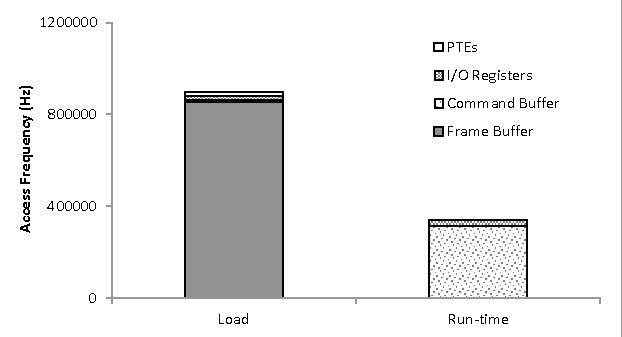
\includegraphics[width=\linewidth]{performance.png}
  \caption{Access patterns of running 3D workloads\cite{183931}}
  \label{fig:performance}
\end{figure}

Figure \ref{fig:performance} shows an average access frequency of running Phoronix 3D workloads on four interfaces: frame buffer, command buffer, PTEs(Page Table Entry) and I/O Registers. At load time, Frame Buffer is dominated, while Run-time is Command Buffer, on the other hands, PTEs and I/O accesses are minor.

As we know, Global graphics memory is mostly the frame buffer, and also used as the command buffer. To achieve better virtualziation performance, we need passthrough the mainly operations, trap and emulate those minor operations, so a better solution is partition global graphic memory and remap it to individual VM, we only let KVM intercepts some specific PTEs and I/O registers by monitor MMIO.  

\subsection{Resource Partitioning}

For virtualization, we need partition physical memory space and MMIO space over PCIe BARs into multiple sections of continuous address space, then assign each to an individual VM. Guest device drivers consider that physical memory space origins from 0, but actual memory access is shifted with a corresponding offset through shadow page tables from hypervisor level. Similarly, GPU channels should be partitioned by multiple sections of the same size for individual VMs\cite{183931}.

\subsection{GPU Memory Virtualization}

The guest graphics driver is unaware of the partitioning, assuming with exclusive ownership: the global graphics memory is contiguous, starting from address zero, so we have to translate between the host view and the guest view before being accessed by the CPU and GPU. The shared shadow global page table keeps the translations from graphics memory frame number to the host memory frame number for all VMs. It is accessible for every VMs. However, only part of the shared global page table can be accessed for one VM to guarantee the isolation.\cite{191581}

The basic solution for keeping shadow page table consistent with guest page table is to write-protect the
shadow page table at all points in time. When a write protection page fault happens, VMM can potentially
trap and emulate and  updates to the guest page table. Therefore huge performance will drop if frequent page table updates. 

\subsection{ GPU Channel Virtualization}

The channel control region size is fixed in different chipset and the number of channels is limit
to different GPUs, so we need a shadow Channel for multiple unknow VMs. The channels should be assigned to virtual machines fairly and isolated among virtual machines. Meanwhile, The device driver assumes that these indexes start from zero. Since the same index cannot be assigned to multiple channels, channel isolation must be supported to multiplex VMs\cite{184002}.

Each GPU channel has its registers, through which the host CPU submits commands to GPU. Channel
registers are saved in GPU virtual address space which is mapped to MMIO. VMM manages all physical channel registers and maintains the mapping between physical and virtual GPU channel registers. Since the virtual channel registers are mapped to MMIO, KVM can intercept the access to them and redirect it to the right physical channel registers. Also the guest GPU driver can dynamically change the index of the channel registers, VMM needs to monitor it and change the mapping in time.

\subsection{GPU Context and its Scheduler}

From above, each context has a dedicated command queue, and a GPU command is submitted to a channel. And the KVM needs maintain a separated context for each virtual machine. Since the guest BAR memory access is intercepted by the hypervisor, the GPU commands submission can be intercepted and added to a queue of context for scheduling. 

The purpose of the virtual GPU scheduler is to share GPU time across VMs fairly. There are usually two GPU schedulers, the Xen default CREDIT, and the BAND (bandwidth-aware non-preemptive device) scheduler from Gdev \cite{Hong:2017:GVS:3101309.3068281}. 

In CREDIT scheduler, each VM maintains a periodically-refreshed budget of credit and a threshold to
prevent over-utilization of the GPU. And the BAND scheduler extends CREDIT by lowering the virtual GPU’s priority only when the budget is exhausted and utilization exceeds the bandwidth.

\section{Conclusion and Future work}

As we know, Software Emulation and API-forwarding could share GPU resources with Multiple VMs, but first one is too slow as all GPU commands needs to be executed by CPU, and API-forwarding needs too much extra work on API level, GPU passthrough could provide a native-close performance, and no need of modification in VM level, however could not be shared by multiple VMs. So Full virtualization performs the best way to partition physical resources and an algorithm to schedule GPU ownership to different VMs.

Full GPU virtualziation provide security isolation by MMIO and Channel virtualization, and high performace based on better Context Scheduler. For future direction, it should be investigated for full virtualization that a dynamic partition method, performance optimization with the help of para-virtualization, better Schedule algorithm, etc. 
\medskip

\bibliographystyle{unsrt}
\bibliography{sample}

\end{document}
